% qual o tempo da apresentação? apresento os apêndices? apresento os trabalhos relacionados? apresento as referências (90)?  
%	Name			:: 	sthlm Beamer Theme  HEAVILY based on the hsrmbeamer theme (Benjamin Weiss)
%	Author			:: 	Mark Hendry Olson (mark@hendryolson.com)
%	Created			::	2013-07-31
%	Updated	    	::	[[April]] 04, 2017 at 16:26:39
%	Version			:: 	2.0.2
%	Email			:: 	hendryolson@gmail.com
%	Website			:: 	http://markolson.se
%	Twitter			:: 	markolsonse
%	Instagram		:: 	markolsonse
%
%	License			:: 	This file may be distributed and/or modified under the
%					GNU Public License.
%
%	Description		::	This presentation is a demonstration of the sthlm beamer
%					theme, which is HEAVILY based on the HSRM beamer theme created by Benjamin Weiss
%					(benjamin.weiss@student.hs-rm.de), which can be found on GitHub
%					<https://github.com/hsrmbeamertheme/hsrmbeamertheme>.  It also borrows heavily
%					from the work of Matthias Vogelgesang, (https://bloerg.net) and his Metropolis Mtheme,
%					<https://github.com/matze/mtheme>.
%
%	Theme			::	newPxFont
%	Options			::	progressbar
%					::	sectionpages
%					::	numfooter
%					::	fullfooter
%					::	dovaligncolumns
%					::	protectframetitle
%					::	greybg
%					::	cblock
%					::	minimal

%-=-=-=-=-=-=-=-=-=-=-=-=-=-=-=-=-=-=-=-=-=-=-=-=
%
%        LOADING DOCUMENT
%
%-=-=-=-=-=-=-=-=-=-=-=-=-=-=-=-=-=-=-=-=-=-=-=-=

\documentclass[newPxFont, numfooter, sectionpages]{beamer}
\usepackage[utf8]{inputenc}
\usetheme{sthlm}
\usepackage{pgfplots}
\pgfplotsset{compat=1.9}
\usepackage{cancel}
\usepackage{amsthm,amsmath}
\usepackage{mathtools}

\usepackage{booktabs}
\usepackage{supertabular}
\usepackage{tabularx}
\usepackage{longtable}
\usepackage{multirow}
\usepackage{hhline}
\usepackage{color, colortbl}

\DeclarePairedDelimiter\abs{\lvert}{\rvert}%
\DeclarePairedDelimiter\norm{\lVert}{\rVert}%
\DeclareMathOperator*{\argmin}{arg\,min}
\DeclareMathOperator*{\argmax}{arg\,max}

\definecolor{lightgray}{gray}{0.8}
\definecolor{Gray}{gray}{0.9}


\title{Discriminative Sensing Based on Signal Processing for Information Security Analysis}
\subtitle{\small{Ph.D. Thesis Qualification}}
\date{\today}
\author{\texttt{Thiago P. de B. Vieira \newline \textbf{Advisor:} João Paulo C. L. da Costa} }
\institute{Universidade de Brasília 
	\par \scriptsize{Departamento de Engenharia Elétrica - ENE/FT}
	\par \scriptsize{Progama de Pós-Graduação em Engenharia Elétrica - PPGEE}
}

\hypersetup{
	pdfauthor = {Thiago P. de B. Vieira},
	pdfsubject = {Discriminative Sensing Based on Signal Processing for Information Security Analysis},
	pdfkeywords = {Signal Processing, Information Security Analysis},
	pdfmoddate= {/home/thiago/dev/projects/discriminative-sensing/docs/thesis/slides},
	pdfcreator = {Sublime and Latex}
}

\begin{document}

%-=-=-=-=-=-=-=-=-=-=-=-=-=-=-=-=-=-=-=-=-=-=-=-=
%
%	TITLE PAGE
%
%-=-=-=-=-=-=-=-=-=-=-=-=-=-=-=-=-=-=-=-=-=-=-=-=
\maketitle
%-=-=-=-=-=-=-=-=-=-=-=-=-=-=-=-=-=-=-=-=-=-=-=-=
%	FRAME: Theme Package Requirements
%-=-=-=-=-=-=-=-=-=-=-=-=-=-=-=-=-=-=-=-=-=-=-=-=
\begingroup
\setbeamercolor{normal text}{fg=\cnDarkGrey,bg=white}


%-=-=-=-=-=-=-=-=-=-=-=-=-=-=-=-=-=-=-=-=-=-=-=-=
%
%	TABLE OF CONTENTS: OVERVIEW
%
%-=-=-=-=-=-=-=-=-=-=-=-=-=-=-=-=-=-=-=-=-=-=-=-=
\section*{Outline}
\begin{frame}{Outline}
	\tableofcontents[hideallsubsections]% For longer presentations use hideallsubsections option
\end{frame}

%-=-=-=-=-=-=-=-=-=-=-=-=-=-=-=-=-=-=-=-=-=-=-=-=
%
%	TABLE OF CONTENTS: OVERVIEW
%
%-=-=-=-=-=-=-=-=-=-=-=-=-=-=-=-=-=-=-=-=-=-=-=-=
\section{Introduction}
%-=-=-=-=-=-=-=-=-=-=-=-=-=-=-=-=-=-=-=-=-=-=-=-=
%	FRAME: Motivation
%-=-=-=-=-=-=-=-=-=-=-=-=-=-=-=-=-=-=-=-=-=-=-=-=
\begin{frame}[c]{Motivation}
	It is necessary investments to detect \textbf{novel attacks and their variations}
	\begin{itemize}
		\item Signal processing schemes have being applied to detect malicious traffic;		
	\end{itemize}
	Secure mobile cloud architecture is challenging, specially in \textbf{offline mode}
	\begin{itemize}
		\item Signal processing can be applied to \textbf{behavioral analysis of mobile apps in offline mode};		
	\end{itemize}
\end{frame}
%-=-=-=-=-=-=-=-=-=-=-=-=-=-=-=-=-=-=-=-=-=-=-=-=
%	FRAME: Motivation
%-=-=-=-=-=-=-=-=-=-=-=-=-=-=-=-=-=-=-=-=-=-=-=-=
\begin{frame}[c]{Motivation}
	\textbf{Fraud detection} of \textbf{Mobile Money Transactions} has been motivating investments
	\begin{itemize}
		\item The \textbf{extraction of relevant information} from \textbf{raw or big} data is useful for classification problems and for security analysis.;
		\item Imbalanced data is challenging for classification related to anomaly detection, novelty detection, fraud detection and attack detection;
		\item \textbf{Tensor-based} algorithms for \textbf{dictionary learning} can improve \textbf{discriminative sensing} for classification in information security analysis;
	\end{itemize}
\end{frame}
%-=-=-=-=-=-=-=-=-=-=-=-=-=-=-=-=-=-=-=-=-=-=-=-=
%	FRAME: Problem Statement
%-=-=-=-=-=-=-=-=-=-=-=-=-=-=-=-=-=-=-=-=-=-=-=-=
\begin{frame}[c]{Problem Statement}
	\textbf{This thesis} outlines the development and evaluation of approaches based on \textbf{signal processing for information security analysis}...
	\begin{itemize}
		\item To make the data \textbf{discriminative} for network attack detection, mobile malicious behavior analysis and fraud detection in mobile money transactions.
	\end{itemize}
\end{frame}
%-=-=-=-=-=-=-=-=-=-=-=-=-=-=-=-=-=-=-=-=-=-=-=-=
%	FRAME: Problem Statement
%-=-=-=-=-=-=-=-=-=-=-=-=-=-=-=-=-=-=-=-=-=-=-=-=
\begin{frame}[c]{Problem Statement}
	We propose an approach based on \textbf{signal processing techniques for detection of malicious traffic in computer networks}
	\begin{itemize}
		\item Signal processing formulation as legitimate traffic, malicious traffic and noise;
		\item MOS and eigenvalue analysis are applied to network attack detection;
		\item Eigen similarity analysis identify accurate time and network ports under attack;
		\item Evaluation through experimental scenario and the DARPA 1998 dataset.
	\end{itemize}
\end{frame}
%-=-=-=-=-=-=-=-=-=-=-=-=-=-=-=-=-=-=-=-=-=-=-=-=
%	FRAME: Problem Statement
%-=-=-=-=-=-=-=-=-=-=-=-=-=-=-=-=-=-=-=-=-=-=-=-=
\begin{frame}[c]{Problem Statement}
	This thesis also proposes an \textbf{approach malicious behavior detection in mobile apps}
	\begin{itemize}
		\item An architecture for mobile security analysis;
		\item Offline user behavior analysis based on MOS;
		\item Scenario analysis for feature selection;
		\item Processing time evaluation in mobile devices.
	\end{itemize}
\end{frame}
%-=-=-=-=-=-=-=-=-=-=-=-=-=-=-=-=-=-=-=-=-=-=-=-=
%	FRAME: Problem Statement
%-=-=-=-=-=-=-=-=-=-=-=-=-=-=-=-=-=-=-=-=-=-=-=-=
\begin{frame}[c]{Problem Statement}
	We also propose a \textbf{tensor-based dictionary learning method for fraud detection from imbalanced data} 
	\begin{itemize}
		\item To evidentiate the \textbf{discriminative sensing of a fraud detection dataset};
		\item Sparse representation based classification (SRC) through learning a tensor-based dictionary;
		\item Apply the learned dictionaries to reconstruct a test signal and classify it as fraud or legitimate;
		\item Classify fraud classification of mobile money transactions according to the reconstruction error.
	\end{itemize}
\end{frame}
%-=-=-=-=-=-=-=-=-=-=-=-=-=-=-=-=-=-=-=-=-=-=-=-=
%	FRAME: Contributions
%-=-=-=-=-=-=-=-=-=-=-=-=-=-=-=-=-=-=-=-=-=-=-=-=
% \begin{frame}{Contributions}
% 	\begin{enumerate}
% 		\item An approach based on \textbf{eigen similarity analysis} for extracting detailed information about accurate time and network ports under network attack;
% 		\item Computational \textbf{complexity analysis} of the proposed framework;
% 		\item An architecture and techniques for \textbf{offline behavioral analysis} of a corporate mobile client security architecture;
% 		\item A \textbf{tensor-based dictionary learning} approach for \textbf{fraud detection} in mobile payment transactions;
% 	\end{enumerate}
% \end{frame}


%-=-=-=-=-=-=-=-=-=-=-=-=-=-=-=-=-=-=-=-=-=-=-=-=
%
%	SECTION: Model Order Selection and Eigen Similarity based Framework for Detection and Identification of Network Attacks
%
%-=-=-=-=-=-=-=-=-=-=-=-=-=-=-=-=-=-=-=-=-=-=-=-=
\section{Model Order Selection and Eigen Similarity based Framework for Detection and Identification of Network Attacks}
%-=-=-=-=-=-=-=-=-=-=-=-=-=-=-=-=-=-=-=-=-=-=-=-=
%	FRAME: Introduction
%-=-=-=-=-=-=-=-=-=-=-=-=-=-=-=-=-=-=-=-=-=-=-=-=
\begin{frame}[c]{Introduction}
	\begin{itemize}
		\item We model the network traffic as a signal processing formulation (\textbf{legitimate traffic, malicious traffic and noise});
		\item The proposed technique is based on eigenvalue analysis, model order selection (MOS) and similarity analysis;
		\item MOS and eigenvalue analysis are applied to detect time frames under attack;
		\item Eigen similarity analysis for extracting detailed time and network ports under attack;
		\item We conduct a performance evaluation for complexity analysis and processing time.
	\end{itemize}
\end{frame}
%-=-=-=-=-=-=-=-=-=-=-=-=-=-=-=-=-=-=-=-=-=-=-=-=
%	FRAME: Related works
%-=-=-=-=-=-=-=-=-=-=-=-=-=-=-=-=-=-=-=-=-=-=-=-=
\begin{frame}[c]{Related works}
	
	\begin{itemize}
		\item Classical methods typically employ data mining [39, 34, 70] and regular file analysis [76] to detect patterns that indicate the presence of specific attacks in network traffic;
		\item Callegari \emph{et al} [104] propose a PCA-based method for identifying the traffic flows responsible for an anomaly detected at the aggregate level and evaluated their proposal through a dataset with synthetic anomalies added in the data. However, Callegari \emph{et al} \textbf{focus on flood attack detection}, not addressing probe attack detection, and their approach relies on \textbf{visual analysis}.
	\end{itemize}
	
\end{frame}
%-=-=-=-=-=-=-=-=-=-=-=-=-=-=-=-=-=-=-=-=-=-=-=-=
%	FRAME: Related works
%-=-=-=-=-=-=-=-=-=-=-=-=-=-=-=-=-=-=-=-=-=-=-=-=
\begin{frame}[c]{Related works}
	
	\begin{itemize}
		\item Lee \emph{et al.} [61] propose OverSampling PCA, determines the \textbf{anomaly} according to the variation of \textbf{eigenvector by similarity analysis and over sampling}. We apply \textbf{MOS for attack detection} and \textbf{similarity analysis for identification} of time and ports under attack;
		\item Lu and Ghorbani [63] proposed a \textbf{network anomaly} detection model based on \textbf{network flow, wavelet approximation, and system identification theory}. However, their work requires a \textbf{training} and presents \textbf{limitations} on identification of behaviors without \textbf{significant outliers}.
	\end{itemize}
	
\end{frame}
%-=-=-=-=-=-=-=-=-=-=-=-=-=-=-=-=-=-=-=-=-=-=-=-=
%	FRAME: Datasets
%-=-=-=-=-=-=-=-=-=-=-=-=-=-=-=-=-=-=-=-=-=-=-=-=
\begin{frame}{Datasets}
	
	We focus on \textbf{probe} and \textbf{flooding} attacks;

	Two scenarios: 
	\begin{itemize}
		\item A \textbf{synthetic dataset} as a signal superposition of legitimate traffic, noise and malicious traffic;
		\item Selected cases of \textbf{DARPA dataset} that reproduce probe and flooding attacks.
	\end{itemize}

\end{frame}
%-=-=-=-=-=-=-=-=-=-=-=-=-=-=-=-=-=-=-=-=-=-=-=-=
%	FRAME: Data Model
%-=-=-=-=-=-=-=-=-=-=-=-=-=-=-=-=-=-=-=-=-=-=-=-=
\begin{frame}{Data Model}
	
	Network traffic:

	\begin{equation}\label{eq:eq01}
		\boldsymbol{X}^{(q)} = \boldsymbol{U}^{(q)} + \boldsymbol{N}^{(q)} + \boldsymbol{A}^{(q)},
	\end{equation}

	$\boldsymbol{X}^{(q)} \in \mathbb{R}^{M \times N}$ has \emph{M} rows and \emph{N} columns. 

	Each row is a TCP or UDP port, and each column represents time bins (minute)

	Each element $x_{m,n}^{(q)}$ stands for the number of times that the port $m$ appears at the $n$-th minute, at the $q$-th time frame.

\end{frame}
%-=-=-=-=-=-=-=-=-=-=-=-=-=-=-=-=-=-=-=-=-=-=-=-=
%	FRAME: Synthetic Dataset
%-=-=-=-=-=-=-=-=-=-=-=-=-=-=-=-=-=-=-=-=-=-=-=-=
\begin{frame}[c]{Synthetic Dataset}
	
	\begin{figure}[h!]
	     \centering
	     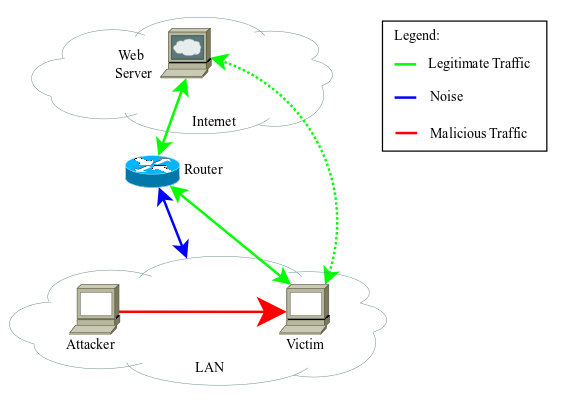
\includegraphics[width=9cm]{../figures/fig09.png}
	     \caption{Scenario to reproduce legitimate traffic, noise, flood and port scan.}
	     \label{fig:2_fig1}
	\end{figure}

\end{frame}
%-=-=-=-=-=-=-=-=-=-=-=-=-=-=-=-=-=-=-=-=-=-=-=-=
%	FRAME: Synthetic Dataset
%-=-=-=-=-=-=-=-=-=-=-=-=-=-=-=-=-=-=-=-=-=-=-=-=
\begin{frame}[c]{Synthetic Dataset}
	
	\begin{figure}[h!]
	     \centering 
	     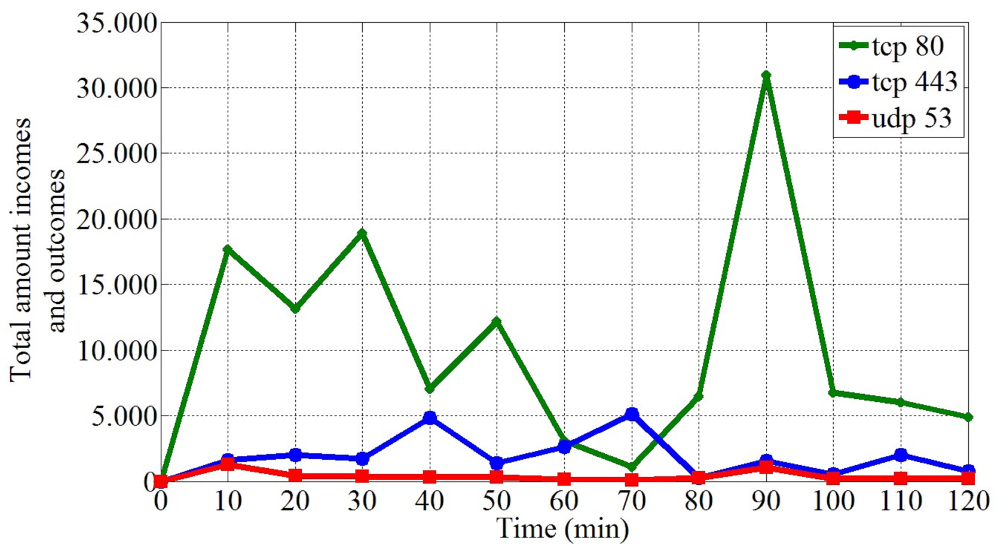
\includegraphics[width=9cm]{../figures/fig03.png}
	     \caption{Traffic from user's operations, that can be characterized by web access, traffic of well-known applications or network protocols.}
	     \label{fig:2_fig3}
	\end{figure}

\end{frame}
%-=-=-=-=-=-=-=-=-=-=-=-=-=-=-=-=-=-=-=-=-=-=-=-=
%	FRAME: Synthetic Dataset
%-=-=-=-=-=-=-=-=-=-=-=-=-=-=-=-=-=-=-=-=-=-=-=-=
\begin{frame}[c]{Synthetic Dataset}
	
	\begin{figure}[h!]
	     \centering 
	     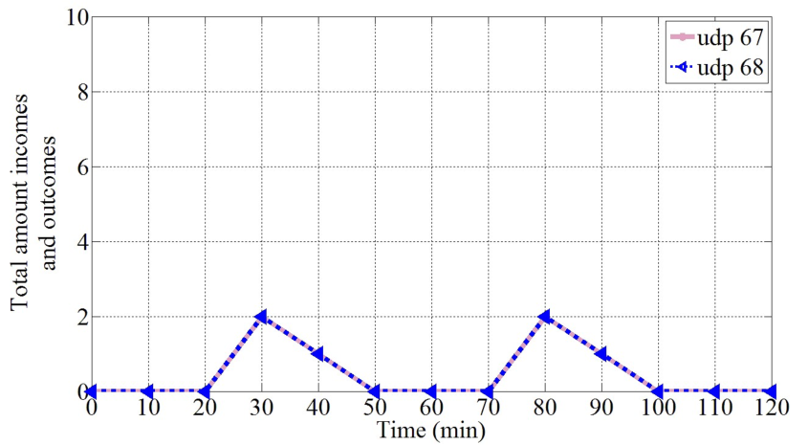
\includegraphics[width=9cm]{../figures/fig04.png}
	     \caption{Network traffic of user independent operations for network management.}
	     \label{fig:2_fig4}
	\end{figure}

\end{frame}
%-=-=-=-=-=-=-=-=-=-=-=-=-=-=-=-=-=-=-=-=-=-=-=-=
%	FRAME: Synthetic Dataset
%-=-=-=-=-=-=-=-=-=-=-=-=-=-=-=-=-=-=-=-=-=-=-=-=
\begin{frame}[c]{Synthetic Dataset}
	
	\begin{figure}[h!]
	     \centering 
	     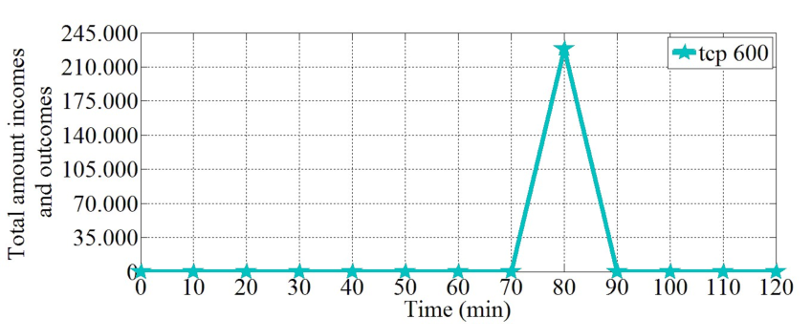
\includegraphics[width=9cm]{../figures/fig05.png}
	     \caption{A large quantity of SYN requests to a target, in order to cause a DoS.}
	     \label{fig:2_fig5}
	\end{figure}

\end{frame}
%-=-=-=-=-=-=-=-=-=-=-=-=-=-=-=-=-=-=-=-=-=-=-=-=
%	FRAME: Synthetic Dataset
%-=-=-=-=-=-=-=-=-=-=-=-=-=-=-=-=-=-=-=-=-=-=-=-=
\begin{frame}[c]{Synthetic Dataset}
	
	\begin{figure}[h!]
	     \centering 
	     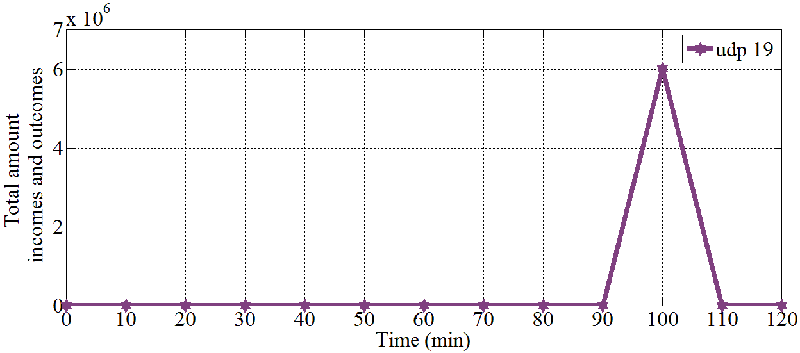
\includegraphics[width=9cm]{../figures/fig06.png}
	     \caption{Large amount of “UDP echo” requests and replies, causing packet flooding.}
	     \label{fig:2_fig6}
	\end{figure}

\end{frame}
%-=-=-=-=-=-=-=-=-=-=-=-=-=-=-=-=-=-=-=-=-=-=-=-=
%	FRAME: Synthetic Dataset
%-=-=-=-=-=-=-=-=-=-=-=-=-=-=-=-=-=-=-=-=-=-=-=-=
\begin{frame}[c]{Synthetic Dataset}
	
	\begin{figure}[h!]
	     \centering 
	     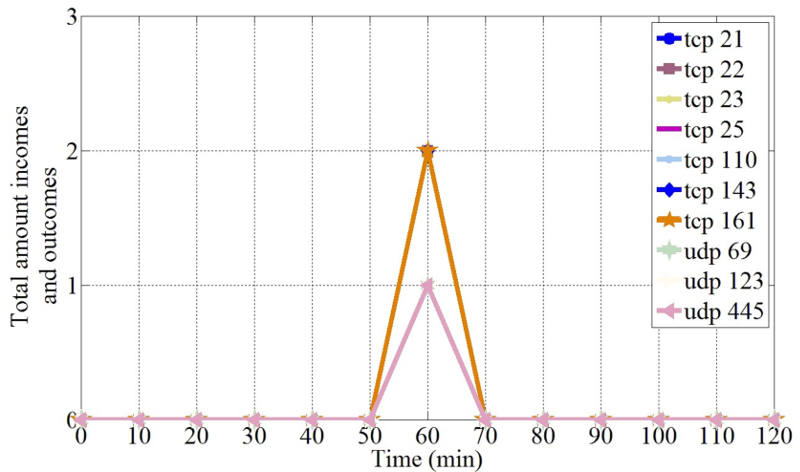
\includegraphics[width=9cm]{../figures/fig07.png}
	     \caption{Connection attempts in order to identify active ports.}
	     \label{fig:2_fig7}
	\end{figure}

\end{frame}
%-=-=-=-=-=-=-=-=-=-=-=-=-=-=-=-=-=-=-=-=-=-=-=-=
%	FRAME: DARPA Dataset
%-=-=-=-=-=-=-=-=-=-=-=-=-=-=-=-=-=-=-=-=-=-=-=-=
\begin{frame}{DARPA Dataset}
	
	\begin{itemize}
		\item 7 weeks of sniffed traffic saved into raw TCPDUMP packet data, from inside and outside origins, with labeled attacks;
		\item The most cases of DoS focus on exploit system vulnerabilities instead of on flooding attack;
		\item We select the cases that reproduce probe and flooding attacks.
	\end{itemize}

\end{frame}
%-=-=-=-=-=-=-=-=-=-=-=-=-=-=-=-=-=-=-=-=-=-=-=-=
%	FRAME: Proposed Framework
%-=-=-=-=-=-=-=-=-=-=-=-=-=-=-=-=-=-=-=-=-=-=-=-=
\begin{frame}{Proposed Framework}
	
	\begin{figure}[h!]
		\centering
	     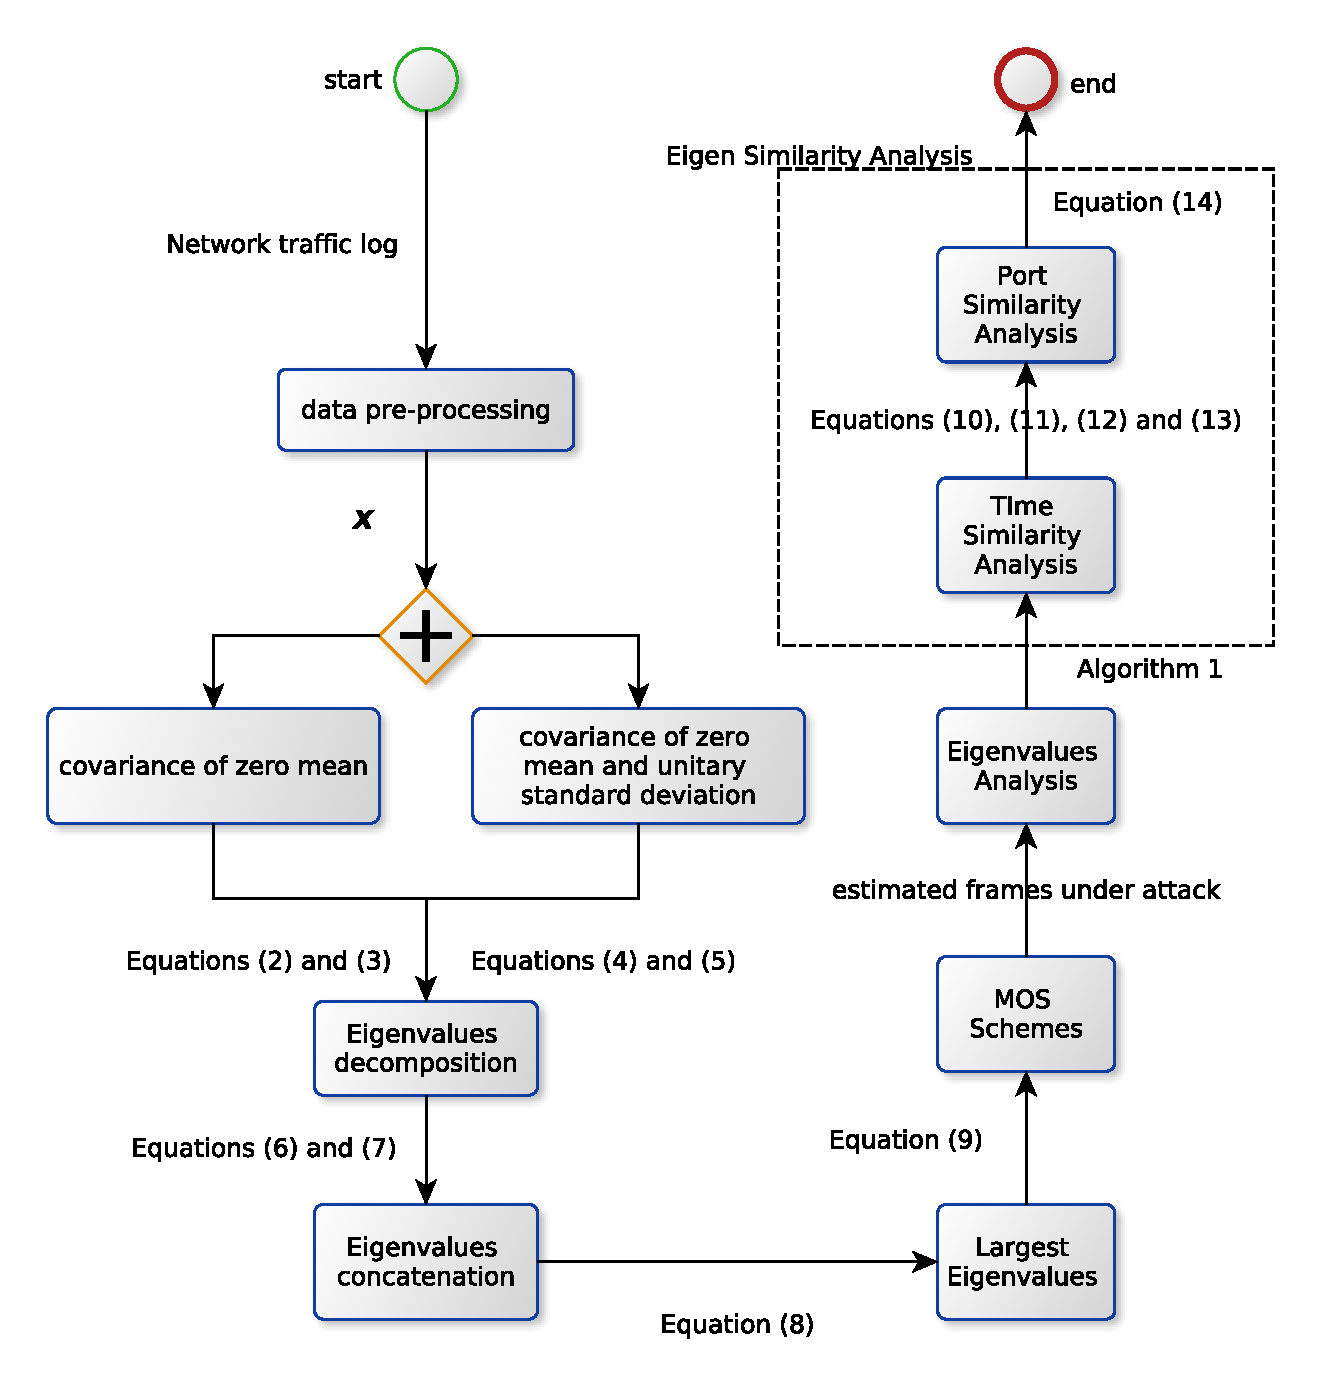
\includegraphics[width=7cm]{../figures/mos_eigen_similarity.eps}
	     \caption{Overview of The Framework for Detection and Identification of Network Attacks.}
	     \label{fig:2_fig80}
	\end{figure}

\end{frame}
%-=-=-=-=-=-=-=-=-=-=-=-=-=-=-=-=-=-=-=-=-=-=-=-=
%	FRAME: Proposed Framework
%-=-=-=-=-=-=-=-=-=-=-=-=-=-=-=-=-=-=-=-=-=-=-=-=
\begin{frame}{Proposed Framework}
	
	For \textbf{flooding} detection, calculate the \textbf{sample covariance matrix} $\boldsymbol{\hat{R}}_{yy}^{(q)}$ of the zero mean samples given by
	\begin{equation}\label{eq:eq02}
		\boldsymbol{y}_{m}^{(q)} = \boldsymbol{x}_{m}^{(q)} - \bar{\boldsymbol{x}}_{m}^{(q)}.
	\end{equation}

	the sample covariance matrix $\boldsymbol{\hat{R}}_{yy}^{(q)}$ can be calculated as follows
	\begin{equation}\label{eq:eq03}
		\boldsymbol{\hat{R}}_{yy}^{(q)} = \frac{1}{N}\boldsymbol{Y}^{(q)}\boldsymbol{Y}^{(q)^{\rm T}}.
	\end{equation}

\end{frame}
%-=-=-=-=-=-=-=-=-=-=-=-=-=-=-=-=-=-=-=-=-=-=-=-=
%	FRAME: Proposed Framework
%-=-=-=-=-=-=-=-=-=-=-=-=-=-=-=-=-=-=-=-=-=-=-=-=
\begin{frame}{Proposed Framework}
	
	For \textbf{probing} detection, compute the \textbf{sample covariance} $\boldsymbol{\hat{R}}_{zz}^{(q)}$ whose variables have \textbf{zero mean and unitary standard deviation} as follows
	\begin{equation}\label{eq:eq04}
		\boldsymbol{z}_{m}^{(q)} = \frac{\boldsymbol{x}_{m}^{(q)} - \bar{\boldsymbol{x}}_{m}^{(q)}}{\boldsymbol{\sigma}_{m}^{(q)}}.
	\end{equation}

	The sample covariance matrix $\boldsymbol{\hat{R}}_{zz}^{(q)}$ can be calculated via 
	\begin{equation}\label{eq:eq05}
		\boldsymbol{\hat{R}}_{zz}^{(q)} = \frac{1}{N}\boldsymbol{Z}^{(q)}\boldsymbol{Z}^{(q)^{\rm T}}.
	\end{equation}

\end{frame}
%-=-=-=-=-=-=-=-=-=-=-=-=-=-=-=-=-=-=-=-=-=-=-=-=
%	FRAME: Proposed Framework
%-=-=-=-=-=-=-=-=-=-=-=-=-=-=-=-=-=-=-=-=-=-=-=-=
\begin{frame}{Proposed Framework}
	
	we refer to $\boldsymbol{\hat{R}}_{yy}$ and $\boldsymbol{\hat{R}}_{zz}$ as a matrix $\boldsymbol{C}$

	Compute eigenvalue decomposition (EVD) to obtain the vector of eigenvalues $\boldsymbol{e}^{(q)}$ associated with each matrix (time frame $q$), according to (\ref{eq:eq060}).
	\begin{equation}\label{eq:eq06}
	\boldsymbol{C}^{(q)} = \boldsymbol{V}^{(q)}\boldsymbol{\Lambda}^{(q)}\boldsymbol{V}^{(q)^{\rm T}},
	\end{equation}
	\begin{equation}\label{eq:eq060}
	\boldsymbol{e}^{(q)} = \rm diag(\boldsymbol{\Lambda}^{(q)}),
	\end{equation}

	The eigenvalues should be sorted in descending order, i.e., $\lambda_{1}^{(q)} > \lambda_{2}^{(q)} > \lambda_{3}^{(q)} > ... > \lambda_{m}^{(q)}$.

\end{frame}
%-=-=-=-=-=-=-=-=-=-=-=-=-=-=-=-=-=-=-=-=-=-=-=-=
%	FRAME: Proposed Framework
%-=-=-=-=-=-=-=-=-=-=-=-=-=-=-=-=-=-=-=-=-=-=-=-=
\begin{frame}{Proposed Framework}
	
	\begin{equation}\label{eq:eq07}
		\boldsymbol{E} =
		\begin{bmatrix}
			\color{red}\lambda_1^{(1)} & \color{red}\lambda_1^{(2)} & \color{red}\lambda_1^{(3)} & \cdots & \color{red}\lambda_1^{(Q)} \\
			\lambda_2^{(1)} & \lambda_2^{(2)} & \lambda_2^{(3)} & \cdots & \lambda_2^{(Q)} \\
			\lambda_3^{(1)} & \lambda_3^{(2)} & \lambda_3^{(3)} & \cdots & \lambda_3^{(Q)} \\
			\vdots & \vdots & \ddots & \vdots  \\
			\lambda_m^{(1)} & \lambda_m^{(2)} & \lambda_m^{(3)} & \cdots & \lambda_m^{(Q)} \\
		\end{bmatrix}.
	\end{equation}

	\begin{equation}\label{eq:eq08}
		\boldsymbol{e}_{\rm max} = \boldsymbol{E}\{:,1\} = [ \lambda_1^{(1)}, \lambda_1^{(2)} ... \lambda_1^{(Q)}]
	\end{equation}

\end{frame}
%-=-=-=-=-=-=-=-=-=-=-=-=-=-=-=-=-=-=-=-=-=-=-=-=
%	FRAME: MOS Scheme
%-=-=-=-=-=-=-=-=-=-=-=-=-=-=-=-=-=-=-=-=-=-=-=-=
\begin{frame}{MOS Scheme}

	\begin{itemize}
		\item Traditionally the MOS schemes are applied for the eigenvalues of the vector $\boldsymbol{e}^{(q)}$;
		\item $\boldsymbol{e}_{\rm max}$ is sorted in descending order, producing $\sim\boldsymbol{e}_{\rm max}$, that is used as input parameter for MOS schemes, according to $\hat{d} = \rm{MOS}(\sim\boldsymbol{e}_{\rm max})$.
		\item $\hat{d}$ is the estimated number of time frames under attack.
	\end{itemize}
	
\end{frame}
%-=-=-=-=-=-=-=-=-=-=-=-=-=-=-=-=-=-=-=-=-=-=-=-=
%	FRAME: Eigenvalue Analysis
%-=-=-=-=-=-=-=-=-=-=-=-=-=-=-=-=-=-=-=-=-=-=-=-=
\begin{frame}{Eigenvalue Analysis}
	
	Through eigenvalue analysis, we identify the time frames $q$ under attack

	\begin{figure}[h!]
	     \centering 
	     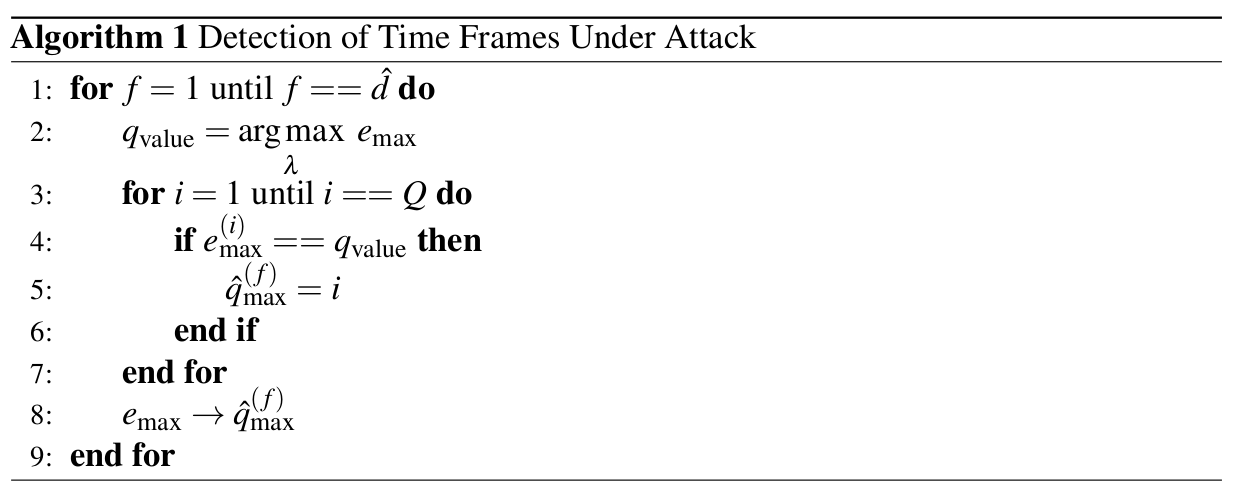
\includegraphics[width=11cm]{alg.png}
	     \label{fig:2_fig9}
	\end{figure}

\end{frame}
%-=-=-=-=-=-=-=-=-=-=-=-=-=-=-=-=-=-=-=-=-=-=-=-=
%	FRAME: Eigenvalue Analysis
%-=-=-=-=-=-=-=-=-=-=-=-=-=-=-=-=-=-=-=-=-=-=-=-=
\begin{frame}{Eigen Similarity Analysis}
	
	The reference eigenvectors $\boldsymbol{v}^{(q)}$ is calculated from the traffic without attack. 

	Each $\boldsymbol{x}^{(\hat{q})}_{(n)}$ vector of each $n$-th minutes of the estimated $\rm{\boldsymbol{\hat{q}}}_{\rm max}$ time frames shall be individually appended into $\boldsymbol{X}^{(q)}$
	\begin{equation}\label{eq:eq12}
		\boldsymbol{X}_{n} = \{\boldsymbol{X}^{(q)} | \boldsymbol{x}^{(\hat{q})}_{(n)}\}.
	\end{equation}

	The resultant $\boldsymbol{X}_{(n)}$ is necessary to obtain $\boldsymbol{v}_{(n)}$, through (\ref{eq:eq06}).

\end{frame}
%-=-=-=-=-=-=-=-=-=-=-=-=-=-=-=-=-=-=-=-=-=-=-=-=
%	FRAME: Eigenvalue Analysis
%-=-=-=-=-=-=-=-=-=-=-=-=-=-=-=-=-=-=-=-=-=-=-=-=
\begin{frame}{Eigen Similarity Analysis}
	
	$s_n$ denotes the absolute similarity degree of the $n$-th minute
	
	$\boldsymbol{v}^{(q)}$ is the most significant eigenvectors

	$\boldsymbol{v}_{(n)}$ is the most significant eigenvectors obtained after append the target $n$-th minute of one network traffic

	For eigen similarity analysis, we evaluate the cosine similarity to identify legitimate and malicious traffic,
	\begin{equation}
		\label{eq:eq11}
		s_n = \frac{\abs{\boldsymbol{v}^{(q)} \cdot \boldsymbol{v}_{(n)}}}{\norm{\boldsymbol{v}^{(q)}}\norm{\boldsymbol{v}_{(n)}}},
	\end{equation}

\end{frame}
%-=-=-=-=-=-=-=-=-=-=-=-=-=-=-=-=-=-=-=-=-=-=-=-=
%	FRAME: Eigenvalue Analysis
%-=-=-=-=-=-=-=-=-=-=-=-=-=-=-=-=-=-=-=-=-=-=-=-=
\begin{frame}{Eigen Similarity Analysis}
	
	We evaluate \textbf{three approaches} for eigen similarity analysis: 
	\begin{itemize}
		\item \textbf{incremental:} concatenates eigenvectors incrementally;
		\item \textbf{individual:} concatenates each eigenvector individually and discards;
		\item \textbf{incremental individualized:} incremental until detect attach and individual after.
	\end{itemize}

\end{frame}
%-=-=-=-=-=-=-=-=-=-=-=-=-=-=-=-=-=-=-=-=-=-=-=-=
%	FRAME: Eigenvalue Analysis
%-=-=-=-=-=-=-=-=-=-=-=-=-=-=-=-=-=-=-=-=-=-=-=-=
\begin{frame}{Eigen Similarity Analysis}
	
	\begin{figure}[h!]
		\centering
	    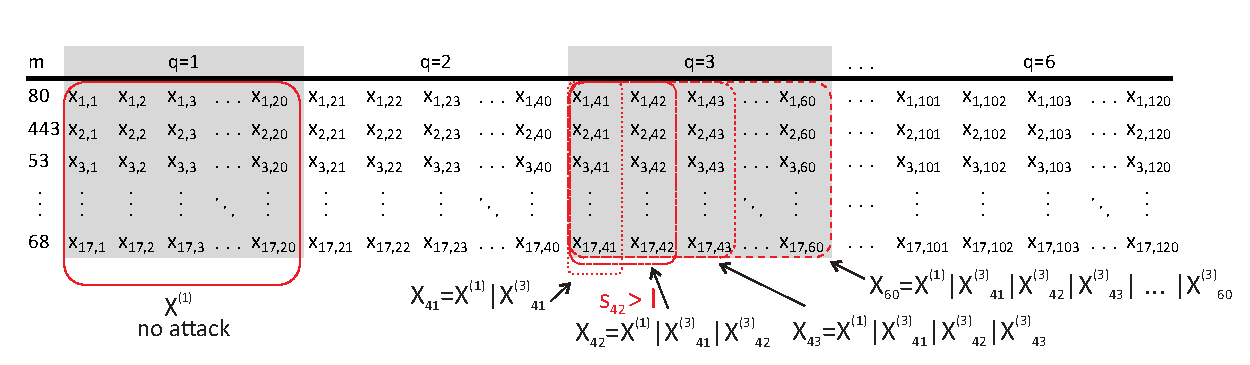
\includegraphics[width=11.5cm]{../figures/incremental.eps}
	    \caption{Traffic selection for incremental approach.}
	    \label{fig:2_fig8}
	\end{figure}

\end{frame}
%-=-=-=-=-=-=-=-=-=-=-=-=-=-=-=-=-=-=-=-=-=-=-=-=
%	FRAME: Eigenvalue Analysis
%-=-=-=-=-=-=-=-=-=-=-=-=-=-=-=-=-=-=-=-=-=-=-=-=
\begin{frame}{Eigen Similarity Analysis}
	
	\begin{figure}[h!]
	     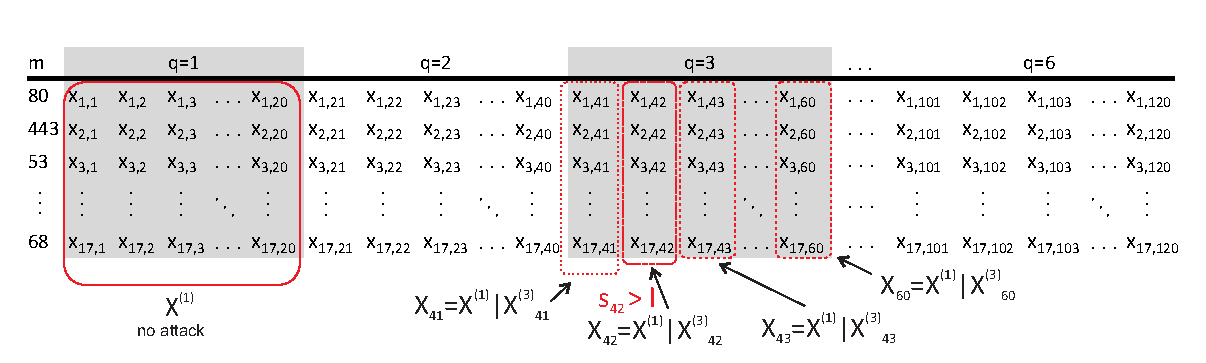
\includegraphics[width=11.5cm]{../figures/individualized.eps}
	     \caption{Traffic selection for individual approach.}
	     \label{fig:2_fig9}
	\end{figure}
\end{frame}
%-=-=-=-=-=-=-=-=-=-=-=-=-=-=-=-=-=-=-=-=-=-=-=-=
%	FRAME: Eigenvalue Analysis
%-=-=-=-=-=-=-=-=-=-=-=-=-=-=-=-=-=-=-=-=-=-=-=-=
\begin{frame}{Eigen Similarity Analysis}
	
	\begin{figure}[h!]
	     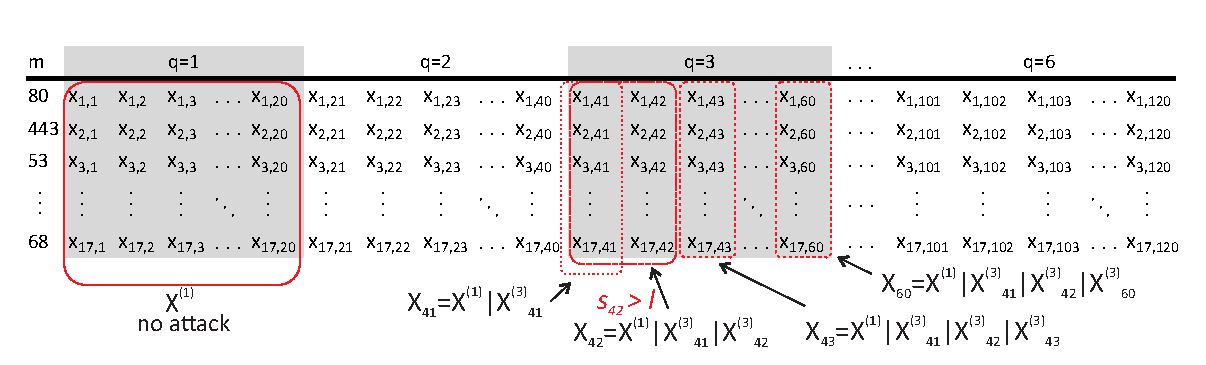
\includegraphics[width=11.5cm]{../figures/incremental_individualized.eps}
	     \caption{Traffic selection for incremental individualized approach.}
	     \label{fig:2_fig2}
	\end{figure}

\end{frame}
%-=-=-=-=-=-=-=-=-=-=-=-=-=-=-=-=-=-=-=-=-=-=-=-=
%	FRAME: Eigenvalue Analysis
%-=-=-=-=-=-=-=-=-=-=-=-=-=-=-=-=-=-=-=-=-=-=-=-=
\begin{frame}{Eigen Similarity Analysis}
	
	For detection of ports under attack, the $\boldsymbol{v}^{(q)}$ last most significant eigenvectors without attack is compared against the $\boldsymbol{v}_{(n)}$ identified as under attack, 

	Evaluate the cosine similarity of each $m$-th port of all $\boldsymbol{\hat{n}}$ minutes.

	\begin{equation}\label{eq:eq15}
		\left\{
		\begin{array}{@{}ll@{}}
			x_{(m,n)} = x^{(\hat{q})}_{(m,\hat{n})} \\
			\\
			s_{m,\hat{n}} = \frac{\abs{\boldsymbol{v}^{(q)} \cdot \boldsymbol{v}_{(m,\hat{n})}}}{\norm{\boldsymbol{v}^{(q)}}\norm{\boldsymbol{v}_{(m,\hat{n})}}},
		\end{array}\right.
	\end{equation}

\end{frame}
%-=-=-=-=-=-=-=-=-=-=-=-=-=-=-=-=-=-=-=-=-=-=-=-=
%	FRAME: Results
%-=-=-=-=-=-=-=-=-=-=-=-=-=-=-=-=-=-=-=-=-=-=-=-=
\begin{frame}{Results}
	
	\begin{table}[h!]
	  \centering
	  \scriptsize
	  \caption{Largest Eigenvalue related to attacks detection}
	  \label{tab:tab3}
	  \begin{tabular}{ c c c c c }
		\toprule
		\multirow{3}{*}{\textbf{Time Frame} $q$} &\multicolumn{4}{c }{\textbf{Vectors GETV}}\\ 
				\hhline{~----}
			&\textbf{Detection of}	 &\textbf{Detection of}	 &\textbf{Detection of}	 &\textbf{Detection of}\\
			&\textbf{\emph{synflood/fraggle}}	 &\textbf{\emph{synflood}}	 &\textbf{\emph{fraggle}}	 &\textbf{\emph{port scan}}\\
		\midrule
		1 &1887545 &1887545 &1887545 &2,0734 \\
		2 &2341327 &2341327 &2341327 &2,1451 \\
		3 &3213867 &3213867 &3213867 &\color{red}10,0718 \\
		4 &\color{red}133238294 &\color{red}133238294 &731229 &2,1620 \\
		5 &\color{red}92384021611 &6367983 &\color{red}92384021611 &2,4253 \\
		6 &708335 &708335 &708335 &1,7948 \\
	    \bottomrule
	  \end{tabular}
	\end{table}

\end{frame}
%-=-=-=-=-=-=-=-=-=-=-=-=-=-=-=-=-=-=-=-=-=-=-=-=
%	FRAME: Results
%-=-=-=-=-=-=-=-=-=-=-=-=-=-=-=-=-=-=-=-=-=-=-=-=
\begin{frame}{Results}
	
	\begin{table}[h!]
	  \centering
	  \tiny
	  \caption{MOS schemes applied to port scan and flood detection}
	  \label{tab:tab4}
	  \begin{tabular}{ c c c c c c c c }
		\toprule
		\multirow{2}{*}{\textbf{Type of analysis} $q$} &\multicolumn{6}{c}{\textbf{MOS schemes (estimated model order $\hat{d}$)}} &{\textbf{(d)}}\\ 
				\hhline{~------~}
			&\textbf{AIC} &\textbf{MDL} &\textbf{EDC} &\textbf{RADOI} &\textbf{EFT} &\textbf{SURE}\\
		\midrule
		Detection of synflood \\(presence of attack) &2 &1 &\textbf{\color{red}1} &5 &\textbf{\color{red}1} &4 &\textbf{\color{red}1} \\
		Detection of synflood \\(absence of attack) &1 &1 &\textbf{\color{red}0} &1 &\textbf{\color{red}0} &3 &\textbf{\color{red}0} \\
		\midrule
		Detection of fraggle \\(presence of attack) &1 &1 &\textbf{\color{red}1} &5 &\textbf{\color{red}1} &4 &\textbf{\color{red}1} \\
		Detection of fraggle \\(absence of attack) &1 &1 &\textbf{\color{red}0} &1 &\textbf{\color{red}0} &3 &\textbf{\color{red}0} \\
		\midrule
		Detection of port scan \\(presence of attack) &1 &1 &\textbf{\color{red}1} &1 &\textbf{\color{red}1} &9 &\textbf{\color{red}1} \\
		Detection of port scan \\(absence of attack) &0 &0 &\textbf{\color{red}0} &1 &\textbf{\color{red}0} &1 &\textbf{\color{red}0} \\
		\midrule
		Detection of synflood/fraggle \\(presence of attack) &2 &2 &\textbf{\color{red}2} &5 &\textbf{\color{red}2} &5 &\textbf{\color{red}2} \\
		Detection of synflood/fraggle \\(absence of attack) &1 &1 &\textbf{\color{red}0} &1 &\textbf{\color{red}0} &3 &\textbf{\color{red}0} \\
	    \bottomrule
	  \end{tabular}
	\end{table}

\end{frame}
%-=-=-=-=-=-=-=-=-=-=-=-=-=-=-=-=-=-=-=-=-=-=-=-=
%	FRAME: Results
%-=-=-=-=-=-=-=-=-=-=-=-=-=-=-=-=-=-=-=-=-=-=-=-=
\begin{frame}{Results}
	
	MOS schemes for probing and flooding attack detection:
	\begin{itemize}
		\item The \textbf{largest eigenvalues visually} indicate the time frame under probing and flooding attack detection;
		\item MOS schemes can estimate it mathematically;
		\begin{itemize}
			\item \textbf{EDC and EFT} estimate \textbf{correctly} the number of attacks $d$;
		\end{itemize}
	\end{itemize}

\end{frame}
%-=-=-=-=-=-=-=-=-=-=-=-=-=-=-=-=-=-=-=-=-=-=-=-=
%	FRAME: Results
%-=-=-=-=-=-=-=-=-=-=-=-=-=-=-=-=-=-=-=-=-=-=-=-=
\begin{frame}{Results}
	
	\begin{table}[h!]
	  \centering
	  \tiny
	  \caption{Eigen Similarity Analysis for Port Scan Detection}
	  \label{tab:tab5}
	  \begin{tabular}{ c c c c c c }
		\toprule
		\multirow{2}{*}{\textbf{Time Frame} $q$} &\multirow{2}{*}{\textbf{Time} $n$}   &\multicolumn{3}{c}{\textbf{Similarity Analysis}} &\multirow{2}{*}{\textbf{Attack?}}\\ 
				\hhline{~~---~}
				& &\textbf{Incremental Individualized} &\textbf{Incremental} &\textbf{Individual}\\
		\midrule
		3 &1 &0.9946 &0.9946 &0.9946 &no \\
		3 &2 &0.9934 &0.9934 &0.9999 &no \\
		3 &3 &0.9912 &0.9912 &0.9999 &no \\
		3 &4 &0.9888 &0.9888 &0.9999 &no \\
		3 &5 &0.9856 &0.9856 &0.9998 &no \\
		3 &6 &0.9840 &0.9840 &0.9999 &no \\
		3 &7 &0.9824 &0.9824 &1.0000 &no \\
		3 &8 &0.9794 &0.9794 &0.9999 &no \\
		3 &9 &0.9673 &0.9673 &0.9926 &no \\
		3 &10 &0.9674 &0.9674 &0.9997 &no \\
		3 &11 &0.9733 &0.9733 &0.9993 &no \\
		3 &12 &0.9702 &0.9702 &0.9993 &no \\
		3 &13 &0.9677 &0.9677 &0.9999 &no \\
		3 &14 &0.9646 &0.9646 &0.9998 &no \\
		3 &15 &\color{red}0.0216 &\color{red}0.0216 &\color{red}0.0276 &\color{red}yes \\
		3 &16 &0.9621 &\color{red}0.0209 &1.0000 &no \\
		3 &17 &0.9611 &\color{red}0.0199 &0.9998 &no \\
		3 &18 &0.9612 &\color{red}0.0191 &0.9999 &no \\
		3 &19 &0.9613 &\color{red}0.0186 &0.9998 &no \\
		3 &20 &0.9638 &\color{red}0.0190 &1.0000 &no \\
	    \bottomrule
	  \end{tabular}
	\end{table}	
	
\end{frame}
%-=-=-=-=-=-=-=-=-=-=-=-=-=-=-=-=-=-=-=-=-=-=-=-=
%	FRAME: Results
%-=-=-=-=-=-=-=-=-=-=-=-=-=-=-=-=-=-=-=-=-=-=-=-=
\begin{frame}{Results}
	
	\begin{table}[h!]
	  \centering
	  \tiny
	  \caption{Eigen Similarity Analysis for Synflood Detection}
	  \label{tab:tab6}
	  \begin{tabular}{ c c c c c c }
		\toprule
		\multirow{2}{*}{\textbf{Time Frame} $q$} &\multirow{2}{*}{\textbf{Time} $n$}   &\multicolumn{3}{c}{\textbf{Similarity Analysis}} &\multirow{2}{*}{\textbf{Attack?}}\\ 
				\hhline{~~---~}
				& &\textbf{Incremental Individualized} &\textbf{Incremental} &\textbf{Individual}\\
		\midrule
		4 &1 &1.0000 &1.0000 &1.0000 &no \\
		4 &2 &0.9999 &0.9999 &1.0000 &no \\
		4 &3 &0.9997 &0.9997 &0.9999 &no \\
		4 &4 &0.9998 &0.9998 &1.0000 &no \\
		4 &5 &0.9965 &0.9965 &0.9908 &no \\
		4 &6 &0.9975 &0.9975 &1.0000 &no \\
		4 &7 &0.9977 &0.9977 &1.0000 &no \\
		4 &8 &0.9980 &0.9980 &1.0000 &no \\
		4 &9 &0.9987 &0.9987 &0.9999 &no \\
		4 &10 &0.9991 &0.9991 &1.0000 &no \\
		4 &11 &\color{red}0.0085 &\color{red}0.0085 &\color{red}0.0284 &\color{red}yes \\
		4 &12 &\color{red}0.0162 &\color{red}0.0120 &\color{red}0.0343 &\color{red}yes \\
		4 &13 &\color{red}0.0248 &\color{red}0.0158 &\color{red}0.0427 &\color{red}yes \\
		4 &14 &\color{red}0.1243 &\color{red}0.0185 &\color{red}0.1041 &\color{red}yes \\
		4 &15 &\color{red}0.0082 &\color{red}0.0162 &\color{red}0.0103 &\color{red}yes \\
		4 &16 &\color{red}0.0404 &\color{red}0.0070 &\color{red}0.0580 &\color{red}yes \\
		4 &17 &\color{red}0.0397 &\color{red}0.0007 &\color{red}0.0573 &\color{red}yes \\
		4 &18 &\color{red}0.0408 &\color{red}0.0042 &\color{red}0.0584 &\color{red}yes \\
		4 &19 &\color{red}0.0408 &\color{red}0.0079 &\color{red}0.0584 &\color{red}yes \\
		4 &20 &\color{red}0.0477 &\color{red}0.0092 &\color{red}0.0757 &\color{red}yes \\
	    \bottomrule
	  \end{tabular}
	\end{table}	
	
\end{frame}
%-=-=-=-=-=-=-=-=-=-=-=-=-=-=-=-=-=-=-=-=-=-=-=-=
%	FRAME: Results
%-=-=-=-=-=-=-=-=-=-=-=-=-=-=-=-=-=-=-=-=-=-=-=-=
\begin{frame}{Results}
	
	\begin{table}[h!]
	  \centering
	  \tiny
	  \caption{Eigen Similarity Analysis for Fraggle Detection}
	  \label{tab:tab7}
	  \begin{tabular}{ c c c c c c }
		\toprule
		\multirow{2}{*}{\textbf{Time Frame} $q$} &\multirow{2}{*}{\textbf{Time} $n$}   &\multicolumn{3}{c}{\textbf{Similarity Analysis}} &\multirow{2}{*}{\textbf{Attack?}}\\ 
				\hhline{~~---~}
				& &\textbf{Incremental Individualized} &\textbf{Incremental} &\textbf{Individual}\\
		\midrule
		5 &1 &1.0000 &1.0000 &1.0000 &no \\
		5 &2 &0.9999 &0.9999 &1.0000 &no \\
		5 &3 &1.0000 &1.0000 &1.0000 &no \\
		5 &4 &0.9999 &0.9999 &1.0000 &no \\
		5 &5 &0.9993 &0.9993 &0.9997 &no \\
		5 &6 &0.9993 &0.9993 &0.9997 &no \\
		5 &7 &0.9994 &0.9994 &1.0000 &no \\
		5 &8 &0.9995 &0.9995 &1.0000 &no \\
		5 &9 &0.9995 &0.9995 &1.0000 &no \\
		5 &10 &0.9995 &0.9995 &1.0000 &no \\
		5 &11 &\color{red}0.0031 &\color{red}0.0031 &\color{red}0.0021 &\color{red}yes \\
		5 &12 &\color{red}0.0019 &\color{red}0.0025 &\color{red}0.0009 &\color{red}yes \\
		5 &13 &\color{red}0.0030 &\color{red}0.0026 &\color{red}0.0020 &\color{red}yes \\
		5 &14 &\color{red}0.0030 &\color{red}0.0027 &\color{red}0.0020 &\color{red}yes \\
		5 &15 &\color{red}0.0030 &\color{red}0.0028 &\color{red}0.0020 &\color{red}yes \\
		5 &16 &\color{red}0.0012 &\color{red}0.0025 &\color{red}0.0002 &\color{red}yes \\
		5 &17 &\color{red}0.0030 &\color{red}0.0026 &\color{red}0.0020 &\color{red}yes \\
		5 &18 &\color{red}0.0030 &\color{red}0.0026 &\color{red}0.0020 &\color{red}yes \\
		5 &19 &\color{red}0.0030 &\color{red}0.0027 &\color{red}0.0020 &\color{red}yes \\
		5 &20 &\color{red}0.0069 &\color{red}0.0023 &\color{red}0.0083 &\color{red}yes \\
	    \bottomrule
	  \end{tabular}
	\end{table}
	
\end{frame}
%-=-=-=-=-=-=-=-=-=-=-=-=-=-=-=-=-=-=-=-=-=-=-=-=
%	FRAME: Results
%-=-=-=-=-=-=-=-=-=-=-=-=-=-=-=-=-=-=-=-=-=-=-=-=
\begin{frame}{Results}
	
	\begin{table}[h!]
	  \centering
	  \tiny
	  \caption{Eigen Similarity Analysis for Detection of Ports Under Port Scan Attack (q=3 and n=15)}
	  \label{tab:tab8}
	  \begin{tabular}{ c c c c }
		\toprule
		\multirow{2}{*}{\textbf{Port} $p$}   &\multicolumn{2}{c}{\textbf{Approaches}} &\multirow{2}{*}{\textbf{Attack?}}\\ 
				\hhline{~--~}
				&\textbf{Incremental Individualized} &\textbf{Individual}\\
		\midrule
		80 &0.9999 &0.9999 &no \\
		443 &0.9999 &0.9999 &no \\
		53 &0.9999 &0.9999 &no \\
		21 &0.9999 &0.9997 &\color{red}yes \\
		22 &\color{red}0.0298 &0.9997 &\color{red}yes \\
		23 &\color{red}0.0298 &0.9997 &\color{red}yes \\
		25 &\color{red}0.0298 &0.9997 &\color{red}yes \\
		110 &\color{red}0.0298 &0.9997 &\color{red}yes \\
		143 &\color{red}0.0298 &0.9997 &\color{red}yes \\
		161 &\color{red}0.0298 &0.9997 &\color{red}yes \\
		69 &\color{red}0.0298 &0.9997 &\color{red}yes \\
		123 &\color{red}0.0298 &0.9997 &\color{red}yes \\
		445 &\color{red}0.0298 &0.9997 &\color{red}yes \\
		600 &0.9999 &0.9999 &no \\
		19 &0.9999 &0.9999 &no \\
		67 &0.9999 &0.9999 &no \\
		68 &0.9999 &0.9999 &no \\
	    \bottomrule
	  \end{tabular}
	\end{table}
	
\end{frame}
%-=-=-=-=-=-=-=-=-=-=-=-=-=-=-=-=-=-=-=-=-=-=-=-=
%	FRAME: Results
%-=-=-=-=-=-=-=-=-=-=-=-=-=-=-=-=-=-=-=-=-=-=-=-=
\begin{frame}{Results}
	
	\begin{table}[h!]
	  \centering
	  \tiny
	  \caption{Eigen Similarity Analysis for Detection of Ports Under Synflood Attack (q=4 and n=11)}
	  \label{tab:tab9}
	  \begin{tabular}{ c c c c }
		\toprule
		\multirow{2}{*}{\textbf{Port} $p$}   &\multicolumn{2}{c}{\textbf{Approaches}} &\multirow{2}{*}{\textbf{Attack?}}\\ 
				\hhline{~--~}
				&\textbf{Incremental Individualized} &\textbf{Individual}\\
		\midrule
		80 &1.0000 &1.0000 &no \\
		443 &1.0000 &1.0000 &no \\
		53 &1.0000 &1.0000 &no \\
		21 &1.0000 &1.0000 &nos \\
		22 &1.0000 &1.0000 &no \\
		23 &1.0000 &1.0000 &no \\
		25 &1.0000 &1.0000 &no \\
		110 &1.0000 &1.0000 &no \\
		143 &1.0000 &1.0000 &no \\
		161 &1.0000 &1.0000 &no \\
		69 &1.0000 &1.0000 &no \\
		123 &1.0000 &1.0000 &no \\
		445 &1.0000 &1.0000 &no \\
		600 &\color{red}0.0077 &\color{red}0.0427 &\color{red}yes \\
		19 &1.0000 &1.0000 &no \\
		67 &1.0000 &1.0000 &no \\
		68 &1.0000 &1.0000 &no \\
	    \bottomrule
	  \end{tabular}
	\end{table}
	
\end{frame}
%-=-=-=-=-=-=-=-=-=-=-=-=-=-=-=-=-=-=-=-=-=-=-=-=
%	FRAME: Results
%-=-=-=-=-=-=-=-=-=-=-=-=-=-=-=-=-=-=-=-=-=-=-=-=
\begin{frame}{Results}
	
	\begin{table}[h!]
	  \centering
	  \tiny
	  \caption{Eigen Similarity Analysis for Detection of Ports Under Fraggle Attack (q=5 and t=11)}
	  \label{tab:tab10}
	  \begin{tabular}{ c c c c }
		\toprule
		\multirow{2}{*}{\textbf{Port} $p$}   &\multicolumn{2}{c}{\textbf{Approaches}} &\multirow{2}{*}{\textbf{Attack?}}\\ 
				\hhline{~--~}
				&\textbf{Incremental Individualized} &\textbf{Individual}\\
		\midrule
		80 &1.0000 &1.0000 &no \\
		443 &1.0000 &1.0000 &no \\
		53 &1.0000 &1.0000 &no \\
		21 &1.0000 &1.0000 &no \\
		22 &1.0000 &1.0000 &no \\
		23 &1.0000 &1.0000 &no \\
		25 &1.0000 &1.0000 &no \\
		110 &1.0000 &1.0000 &no \\
		143 &1.0000 &1.0000 &no \\
		161 &1.0000 &1.0000 &no \\
		69 &1.0000 &1.0000 &no \\
		123 &1.0000 &1.0000 &no \\
		445 &1.0000 &1.0000 &no \\
		600 &1.0000 &1.0000 &no \\
		19 &\color{red}0.0031 &\color{red}0.0004 &\color{red}yes \\
		67 &1.0000 &1.0000 &no \\
		68 &1.0000 &1.0000 &no \\
	    \bottomrule
	  \end{tabular}
	\end{table}
	
\end{frame}
%-=-=-=-=-=-=-=-=-=-=-=-=-=-=-=-=-=-=-=-=-=-=-=-=
%	FRAME: Results
%-=-=-=-=-=-=-=-=-=-=-=-=-=-=-=-=-=-=-=-=-=-=-=-=
\begin{frame}{Results}
	
	For \textbf{time} attack detection:
	\begin{itemize}
		\item \textbf{High similarity} between network traffic \textbf{without attack} (0.9610) and \textbf{low similarity} with \textbf{attack} (0.0276);
		\item The \textbf{incremental} approach produces \textbf{false positive} results;
		\item Capability of \textbf{change detection} based on similarity between legitimate and malicious traffic (flood or probe);
	\end{itemize}
	
	For \textbf{port} attack detection:
	\begin{itemize}
		\item The \textbf{incremental individualized} has more \textbf{sensibility} to anomaly detection;
		\item The \textbf{individual} approach \textbf{was not able} to identify low similarity for ports under attack;
	\end{itemize}
	
\end{frame}
% %-=-=-=-=-=-=-=-=-=-=-=-=-=-=-=-=-=-=-=-=-=-=-=-=
% %	FRAME: Results
% %-=-=-=-=-=-=-=-=-=-=-=-=-=-=-=-=-=-=-=-=-=-=-=-=
% \begin{frame}{Results}
	
% 	Conclusion:
% 	\begin{itemize}
% 		\item \textbf{Incremental individualized can detect} low similarity for all evaluated network attacks, while the \textbf{other approaches presented false positives or low sensibility};
% 		\item This approach is able to \textbf{gradually and incrementally adapt to network traffic changing}.
% 	\end{itemize}

% \end{frame}
%-=-=-=-=-=-=-=-=-=-=-=-=-=-=-=-=-=-=-=-=-=-=-=-=
%	FRAME: Results - DARPA Dataset
%-=-=-=-=-=-=-=-=-=-=-=-=-=-=-=-=-=-=-=-=-=-=-=-=
\begin{frame}{Results - DARPA Dataset}
	
	\begin{table}[!t]
		\caption{Results of the attack detection evaluation}
		\label{tab:tab12}
		\centering
		\scriptsize
		\begin{tabular}{|c|c|c|c|c|}
			\hline \rowcolor{Gray} \begin{tabular}[x]{@{}l@{}}Solution\end{tabular}	& \begin{tabular}[x]{@{}l@{}}Attack Type\end{tabular}	 & \begin{tabular}[x]{@{}l@{}}Metric\end{tabular}	& \begin{tabular}[x]{@{}l@{}}Result\end{tabular} \\ \hline
			Proposed Work	&Flooding	&True Positive	&100.00 \%\\ \hline
			Proposed Work	&Flooding	&False Positive	&60.00 \%\\ \hline
			Proposed Work	&Flooding	&Misclassification	&50.00 \%\\ \hline
			Proposed Work	&Probe	&True Positive	&76.92 \%\\ \hline
			Proposed Work	&Probe	&False Positive	&18.52 \%\\ \hline
			Proposed Work	&Probe	&Misclassification	&32.73 \%\\ \hline
			Callegari \emph{et al}	&Flooding	&True Positive	&82.00 \%\\ \hline
			Callegari \emph{et al}	&Flooding	&False Positive	&-\\ \hline
			Callegari \emph{et al}	&Flooding	&Misclassification	&-\\ \hline
			Lu and Ghorbani	&Overall	&True Positive	&94.67 \%\\ \hline
			Lu and Ghorbani	&Overall	&False Positive	&-\\ \hline
			Lu and Ghorbani	&Overall	&Misclassification	&-\\ \hline
			Lu and Ghorbani	&Portsweep	&True Positive	&50.00 \%\\ \hline
			Lu and Ghorbani	&Portsweep	&False Positive	&-\\ \hline
			Lu and Ghorbani	&Portsweep	&Misclassification	&-\\ \hline
		\end{tabular}
	\end{table}
	
\end{frame}
%-=-=-=-=-=-=-=-=-=-=-=-=-=-=-=-=-=-=-=-=-=-=-=-=
%	FRAME: Results - DARPA Dataset
%-=-=-=-=-=-=-=-=-=-=-=-=-=-=-=-=-=-=-=-=-=-=-=-=
\begin{frame}{Results - DARPA Dataset}
	
	% Misclassification is defined as $\frac{(FN+FP)}{(TP+FP+FN+TN)}$;
	\begin{itemize}
		\item High FP and misclassification due to legitimate traffic be massive (such as an attack) sometimes;
		\item Callegari \emph{et al} is a statistical method, based on PCA, without training or learning methods
		\begin{itemize}
			\item 82 \% while we obtain 100 \%;
			\item FP and misclassification was not evaluated.
		\end{itemize}
		\item Ghorbani's is based on signal processing techniques and uses DARPA
		\begin{itemize}
			\item 94.67 \% and 50.00 \%, while we obtain 100 \% and 76.92 \%;
			\item FP and misclassification was not evaluated.
		\end{itemize}
	\end{itemize}
\end{frame}
%-=-=-=-=-=-=-=-=-=-=-=-=-=-=-=-=-=-=-=-=-=-=-=-=
%	FRAME: Performance Evaluation
%-=-=-=-=-=-=-=-=-=-=-=-=-=-=-=-=-=-=-=-=-=-=-=-=
\begin{frame}{Performance Evaluation}

	Complexity Analysis:
	\begin{itemize}
		\item the proposed framework is $O(N^3 + Q \log Q + \hat{d}Q + N^3)$ and its worst-case running time is $O(N^3)$;
		\item The computational complexity of \textbf{EVD is predominant};
		\item \textbf{However}, the approach \textbf{splits the data into time frames} with period time $N$, which makes possible to \textbf{limit the growth of $N$} even when \textbf{total time is larger} than $N$;		
	\end{itemize}
	
\end{frame}
%-=-=-=-=-=-=-=-=-=-=-=-=-=-=-=-=-=-=-=-=-=-=-=-=
%	FRAME: Performance Evaluation
%-=-=-=-=-=-=-=-=-=-=-=-=-=-=-=-=-=-=-=-=-=-=-=-=
\begin{frame}{Performance Evaluation}
	
	Processing Time Analysis:
	\begin{itemize}
		\item desktop computer with a Intel Core i7-4510U 2.00GHz and 16 GB of RAM;
		\item Network traffic time; 
		\item Frame size denoted as $N$; 
		\item Number of network ports denoted as $M$; 
		\item Mean processing time for eigen analysis based on sample covariance of zero mean (1-time); 
		\item Mean processing time for eigen analysis based on sample covariance of zero mean and unitary standard deviation (2-time); 
		\item Mean processing time for EDC MOS scheme, (3-time).
	\end{itemize}
	
\end{frame}
%-=-=-=-=-=-=-=-=-=-=-=-=-=-=-=-=-=-=-=-=-=-=-=-=
%	FRAME: Performance Evaluation
%-=-=-=-=-=-=-=-=-=-=-=-=-=-=-=-=-=-=-=-=-=-=-=-=
\begin{frame}{Performance Evaluation}
	
	\begin{table}[!t]
		\caption{Processing time of the main steps for anomaly detection}
		\label{tab:11}
		\centering
		\tiny
		\begin{tabular}{|r|r|r|r|r|r|r|}
			\hline \rowcolor{Gray} \begin{tabular}[x]{@{}l@{}}Traffic Time\\(hour)\end{tabular}	& \begin{tabular}[x]{@{}l@{}}Frame Size\\(min)\end{tabular}	 & \begin{tabular}[x]{@{}l@{}}Num. Ports\end{tabular}	& \begin{tabular}[x]{@{}l@{}}1-time\\(ms)\end{tabular}	& \begin{tabular}[x]{@{}l@{}}2-time\\(ms)\end{tabular}	& \begin{tabular}[x]{@{}l@{}}3-time\\(ms)\end{tabular}	\\ \hline
			16	& 10	& 17	& 0.7900	& 0.8100	& 0.0650\\ \hline
			16	& 20	& 17	& 0.5250	& 0.5950	& 0.0100\\ \hline
			16	& 60	& 17	& 0.9700	& 1.1400	& 0.0250\\ \hline
			16	& 120	& 17	& 0.6050	& 0.6100	& 0.0050\\ \hline
			16	& 60	& 34	& 1.2750	& 1.2200	& 0.0050\\ \hline
			16	& 120	& 34	& 1.1200	& 1.1700	& 0.0050\\ \hline
			20	& 10	& 17	& 2.7950	& 2.8950	& 1.1000\\ \hline
			20	& 20	& 17	& 2.0700	& 2.0200	& 0.3500\\ \hline
			20	& 60	& 17	& 1.0250	& 1.0450	& 0.0650\\ \hline
			20	& 120	& 17	& 1.0000	& 1.0700	& 0.0350\\ \hline
			20	& 60	& 34	& 2.9650	& 3.2100	& 0.0400\\ \hline
			20	& 120	& 34	& 2.9950	& 3.1150	& 0.0200\\ \hline
			22	& 10	& 17	& 4.7250	& 4.0850	& 1.4600\\ \hline
			22	& 20	& 17	& 2.3200	& 2.6800	& 0.2450\\ \hline
			22	& 60	& 17	& 1.0700	& 1.1200	& 0.0300\\ \hline
			22	& 120	& 17	& 0.9900	& 1.0500	& 0.0250\\ \hline
			22	& 60	& 34	& 3.0850	& 3.1250	& 0.0650\\ \hline
			22	& 120	& 34	& 2.8100	& 2.9600	& 0.0250\\ \hline
		\end{tabular}
	\end{table}
	
\end{frame}
%-=-=-=-=-=-=-=-=-=-=-=-=-=-=-=-=-=-=-=-=-=-=-=-=
%	FRAME: Performance Evaluation
%-=-=-=-=-=-=-=-=-=-=-=-=-=-=-=-=-=-=-=-=-=-=-=-=
\begin{frame}{Performance Evaluation}

	Processing Time Analysis:
	\begin{itemize}
		\item The processing time increases according to traffic time, but the \textbf{worst} processing time is \textbf{4.7250 milliseconds};
		\item The processing time \textbf{increases} with the frame size $N$ \textbf{decreasing};
		\item The number of ports $M$ increases the processing time.
	\end{itemize}
	
\end{frame}


%-=-=-=-=-=-=-=-=-=-=-=-=-=-=-=-=-=-=-=-=-=-=-=-=
%	SECTION: Offline Mode for Corporate Mobile Client Security Architecture
%-=-=-=-=-=-=-=-=-=-=-=-=-=-=-=-=-=-=-=-=-=-=-=-=
\section{Offline Mode for Corporate Mobile Client Security Architecture}
\label{Blocks}
%-=-=-=-=-=-=-=-=-=-=-=-=-=-=-=-=-=-=-=-=-=-=-=-=
%	FRAME: Introduction
%-=-=-=-=-=-=-=-=-=-=-=-=-=-=-=-=-=-=-=-=-=-=-=-=
\begin{frame}[c]{Introduction}
	\begin{itemize}
		\item We model the network traffic as a signal processing formulation (\textbf{legitimate traffic, malicious traffic and noise});
		\item The proposed technique is based on eigenvalue analysis, model order selection (MOS) and similarity analysis;
		\item MOS and eigenvalue analysis are applied to detect time frames under attack;
		\item Eigen similarity analysis for extracting detailed time and network ports under attack;
		\item We conduct a performance evaluation for complexity analysis and processing time.
	\end{itemize}
\end{frame}

%-=-=-=-=-=-=-=-=-=-=-=-=-=-=-=-=-=-=-=-=-=-=-=-=
%
%	SECTION: Tensor-based Discriminative Sensing for Fraud Detection
%
%-=-=-=-=-=-=-=-=-=-=-=-=-=-=-=-=-=-=-=-=-=-=-=-=
\section{Tensor-based Discriminative Sensing for Fraud Detection}
%-=-=-=-=-=-=-=-=-=-=-=-=-=-=-=-=-=-=-=-=-=-=-=-=
%	FRAME: Introduction
%-=-=-=-=-=-=-=-=-=-=-=-=-=-=-=-=-=-=-=-=-=-=-=-=
\begin{frame}[c]{Introduction}
	\begin{itemize}
		\item We model the network traffic as a signal processing formulation (\textbf{legitimate traffic, malicious traffic and noise});
		\item The proposed technique is based on eigenvalue analysis, model order selection (MOS) and similarity analysis;
		\item MOS and eigenvalue analysis are applied to detect time frames under attack;
		\item Eigen similarity analysis for extracting detailed time and network ports under attack;
		\item We conduct a performance evaluation for complexity analysis and processing time.
	\end{itemize}
\end{frame}


%-=-=-=-=-=-=-=-=-=-=-=-=-=-=-=-=-=-=-=-=-=-=-=-=
%
%	SECTION: Conclusion and Future Work
%
%-=-=-=-=-=-=-=-=-=-=-=-=-=-=-=-=-=-=-=-=-=-=-=-=
\section{Conclusion and Future Work}
%-=-=-=-=-=-=-=-=-=-=-=-=-=-=-=-=-=-=-=-=-=-=-=-=
%	FRAME: Introduction
%-=-=-=-=-=-=-=-=-=-=-=-=-=-=-=-=-=-=-=-=-=-=-=-=
\begin{frame}[c]{Introduction}
	\begin{itemize}
		\item We model the network traffic as a signal processing formulation (\textbf{legitimate traffic, malicious traffic and noise});
		\item The proposed technique is based on eigenvalue analysis, model order selection (MOS) and similarity analysis;
		\item MOS and eigenvalue analysis are applied to detect time frames under attack;
		\item Eigen similarity analysis for extracting detailed time and network ports under attack;
		\item We conduct a performance evaluation for complexity analysis and processing time.
	\end{itemize}
\end{frame}

\end{document}